\begin{frame}{Illustration avec un outil de tous les jours : Wikipédia}
Définie comme une encyclopédie collaborative, en ligne, à laquelle tout le monde peut donc gratuitement accéder et librement contribuer.\\
Revenir sur l'opposition fondamentale que certains établissent entre les modèles imprimés et le modèle numérique, afin de démontrer deux choses :
\begin{itemize}
    \item Général: le passage de l'imprimé au numérique n'est pas la révolution numérique que l'on veut faire croire.
    
    \item Cas particulier de l'encyclopédie: ce n'est pas la disparition d'un savoir faire, mais l'apparition d'un nouveau modèle épistémique, un modèle étroitement lié au fonctionnement même des media imprimés et numériques.
\end{itemize}

\end{frame}

\begin{frame}{D'\textit{Universalis} à \textit{Wikipédia} : deux modèles et protocoles éditoriaux numériques pour deux conceptions encyclopédiques opposées}
    
    \begin{columns}[T,onlytextwidth]
\column{0.50\linewidth}
\textbf{Modèle homothétique}
\centering

\includegraphics[width=.80\columnwidth]{05_Axe1_protocoles/images/universalis.png}
\begin{itemize}
    \item Acces fermé par une plateforme institutionnel restreinte
    \item Autorité de l'expert
    \item Stabilité et clôture du texte
\end{itemize}
\column{0.50\linewidth}
\textbf{Modèle éditorialisé}
\centering
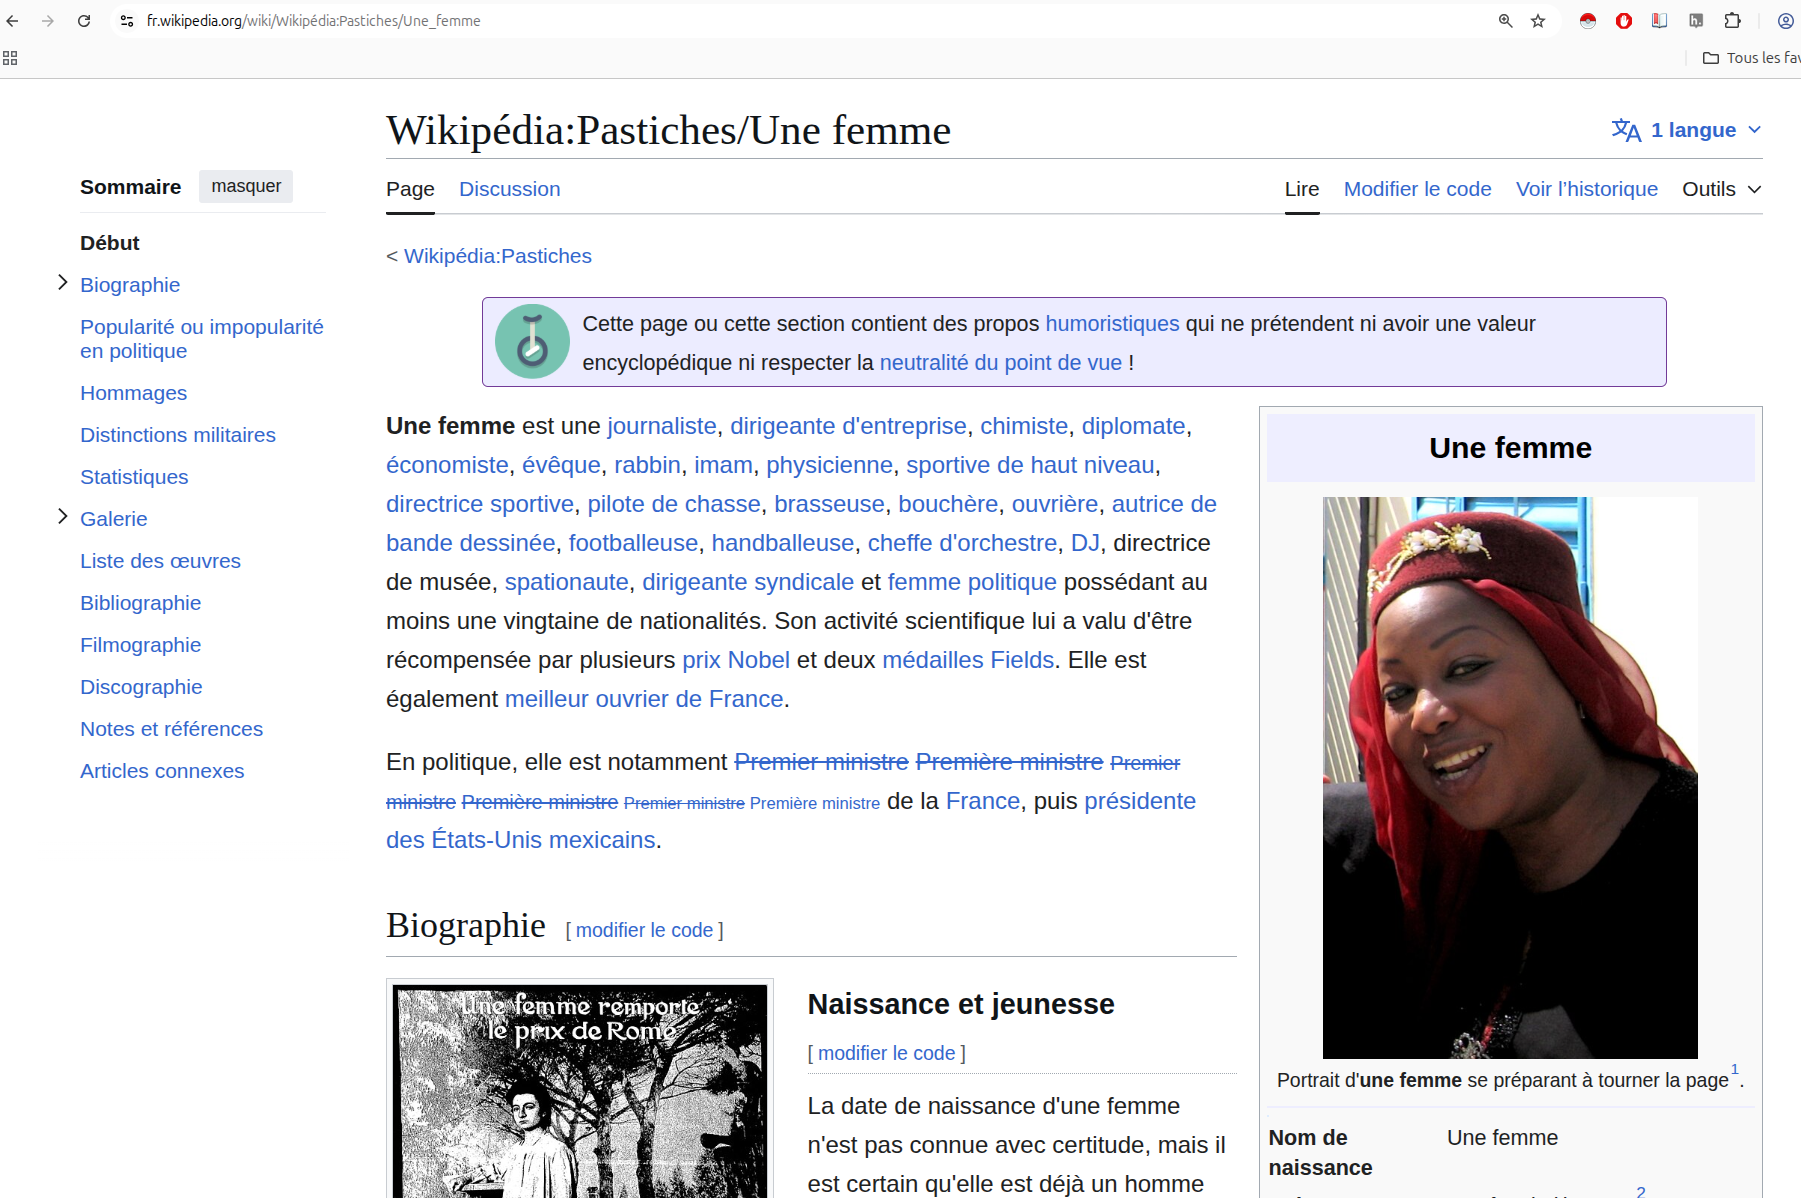
\includegraphics[width=.80\columnwidth]{05_Axe1_protocoles/images/wikipedia-une-femme.png}
\begin{itemize}
    \item Écriture processuelle : ouverture dans le temps
    \item Écriture collective
    \item Accès ouvert et gratuit, ancrage dans le web
\end{itemize}
\end{columns}
\end{frame}

\begin{frame}{Le modèle Universalis : une culture de l'imprimé}
    \begin{columns}[T,onlytextwidth]
\column{0.50\linewidth}

\begin{itemize}
    \item Existe depuis 1966
    \item Publiée par la société d'édition Encyclopædia Universalis SA
    \item Née sur un support imprimé.
\end{itemize}
\column{0.50\linewidth}
\centering

\includegraphics[width=6cm]{05_Axe1_protocoles/images/universalis_livre.png}
\end{columns}

\end{frame}

\begin{frame}{Le modèle Universalis : une culture de l'imprimé}
\begin{itemize}
    \item Un éditeur en chef
    \item Un réseau "d'experts" (universitaires)
    \item Une chaîne éditoriale séquentielle (écriture -> correction -> publication)
    \item Des articles signés, relativement stables
\end{itemize}    
\end{frame}

\begin{frame}{Le modèle Universalis : une culture de l'imprimé}
\begin{center}
    
\includegraphics[width=4cm]{05_Axe1_protocoles/images/universalis_cdrom.png}
    \hspace{2em}
    
\includegraphics[width=7cm]{05_Axe1_protocoles/images/universalis_web.png}
\end{center}
\end{frame}

\begin{frame}{Deux acteurs importants}

\begin{block}{L'éditeur, figure centrale garante du respect du protocole}
    \begin{itemize}
        \item Garant de la fiabilité des contenus (gère les auteurs, vérifie les références)
        \item Garant de la mise en forme (gestion iconographique, cartes mentales)
    \end{itemize}
\end{block}
    
\begin{block}{L'auteur, guidé par le protocole éditorial}
    \begin{itemize}
        \item Des auteurs sollicités pour leur expertise (universitaires, professeurs)
        \item Des articles commandés (tâches d'écriture définies en amont dans un cahier des charges)
        \item Une attention portée à l'écriture (uniformisation du style, travail de synthèse et de vulgarisation)
    \end{itemize}
\end{block}
\end{frame}

\begin{frame}{Universalis en ligne : un modèle "homothétique"}
    \centering
    
\includegraphics[width=12cm]{05_Axe1_protocoles/images/universalis_ex.png}
\end{frame}

\begin{frame}{Un peu d'histoire : de Nupedia à Wikipédia, histoire d'un échec}

\begin{itemize}
    \item \textbf{Content Management System}: programme permettant de créer un site internet sans que les utilisateurs n'aient besoin de compétences en informatiques
    \item \textbf{Wiki} = logiciel permettant la création, la modification et l'illustration collaboratives de pages à l'intérieur d'un site web.
\end{itemize}

\end{frame}

\begin{frame}{Le projet Nupedia (2000 - 2003)}
    \begin{columns}
        \column{.30\linewidth}
        \begin{itemize}
            \item Fondateur: Jimmy Wales
            \item Éditeur en chef: Larry Sanger
        \end{itemize}
        \column{.60\linewidth}
        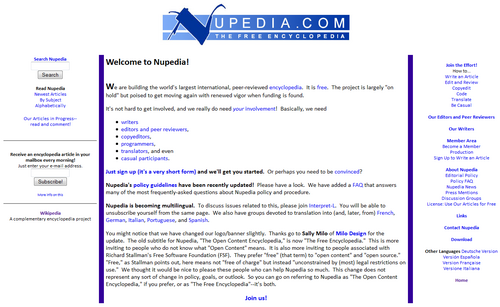
\includegraphics[width=.90\textwidth]{05_Axe1_protocoles/images/Nupedia_main_page.png}
    \end{columns}
\end{frame}

\begin{frame}{Nupedia : l'échec du protocole homothétique}
    \centering
    {\small
    \textit{Wikipédia n’est pas née radicale. Avant elle, Nupédia, la première encyclopédie en ligne lancée par Jimmy Wales au sein de sa société, Bomis, recouvrait une forme très traditionnelle. Un éditeur en chef, Larry Sanger, recruté à cet effet, surveillait et validait les contributions d’auteurs choisis pour leur expertise (Levrel, 2006). Le processus d’édition et de validation des articles était très rigoureux et s’appuyait sur un collège d’experts certifiés. La petite histoire raconte que Larry Sanger vérifiait que les contributeurs aient bien un doctorat (PhD), en leur demandant de lui envoyer leur diplôme par fax (Lih, 2009, p. 38)}}\\
    \vspace{1em}
    \textbf{Dominique Cardon, \textit{"Surveiller sans punir. La gouvernance de Wikipédia", Wikipédia, objet scientifique non identifié}, édité par Lionel Barbe et al., Presses universitaires de Paris Nanterre, 2015.}
\end{frame}

\begin{frame}{Nupedia, l'encyclopédie "incunable" ?}
    \centering
    {\small
    \textit{Au bout d’un an de fonctionnement, Nupédia ne parviendra pas à réunir plus de 20 articles : le processus était long, l’investissement des experts dilettante, le financement du projet fragile. Nupédia aurait très vite été oublié si, à titre expérimental, Larry Sanger et Jimmy Wales n’avaient décidé en janvier 2001 de lancer un wiki destiné à élaborer des ébauches d’articles pour Nupédia en permettant aux experts et à d’autres, d’écrire, de corriger et d’annoter les textes. À une vitesse stupéfiante, Wikipédia, simple « bac à sable » de Nupédia, va très vite se développer en suscitant l’attention d’internautes non experts, pendant que Nupédia sera définitivement déserté.}}\\
    \vspace{1em}
    \textbf{Dominique Cardon, \textit{"Surveiller sans punir. La gouvernance de Wikipédia", Wikipédia, objet scientifique non identifié}, édité par Lionel Barbe et al., Presses universitaires de Paris Nanterre, 2015.}

\end{frame}

\begin{frame}{De Nupedia à Wikipedia}
    \begin{block}{Une évolution du protocole éditorial...}
        \begin{itemize}
            \item Le CMS Wiki comme technologie de l'intellect
            \item Un modèle "horizontal" mais une gouvernance très stricte
            \item Un modèle extrêmement régulé (règles de contribution, de mise en forme, protocoles éditoriaux)
        \end{itemize}
    \end{block}

    \begin{block}{... et du concept de connaissance}
        \begin{itemize}
            \item Vers un principe de vérifiabilité
            \item Vers des communs de la connaissance
            \item Vers une autorité partagée
        \end{itemize}
    \end{block}
\end{frame}

\begin{frame}{Le CMS wiki : une interface régulatrice du collectif}
   Dominique Cardon (sociologue) explique que: le CMS (plateforme reposant sur un protocole éditorial co-construit entre les utilisateurs) suppose une régulation plus ou moins forte des comportements et des publications.\\
\begin{block}{}
\centering
     \textit{Les wikipédiens "ont choisi de confier à l’interface elle-même et aux règles de l’encyclopédie le soin de prendre en charge et de garantir que les comportements des wikipédiens soient bien orientées vers le savoir épistémique."}
\end{block}

\textrightarrow{} Le dispositif wiki fait agir les usagers en « wikipédiens » au profit du projet encyclopédique. 
\end{frame}

\begin{frame}{Le CMS wiki : une interface régulatrice du collectif}
\begin{itemize}
    \item Interactions avec les autres rédacteurs, les notifications apposées sur leurs contributions \textrightarrow{} les participants plient, adaptent et ajustent leurs comportements aux règles collectives.
    \item Ce sont les ajustements mutuels qui permettent aux personnes d'intéragir sur le wiki
    \item Interface de Wikipédia \textrightarrow{} contiguïté serrée entre l'espace des pratiques et celui des normes de la pratique.
\end{itemize} 
(Tiré de Dominique Cardon, \textit{"Surveiller sans punir. La gouvernance de Wikipédia", Wikipédia, objet scientifique non identifié}, édité par Lionel Barbe et al., Presses universitaires de Paris Nanterre, 2015.)
\end{frame}

